\section{Results}\label{sec:results}

CKG results are final across all 44 domains (7,588 queries). RAG results
are final across 40 of 44 domains (6,844 queries); the remaining 4 domains
(\texttt{asl-book}, \texttt{infographics}, \texttt{machine-learning-textbook},
\texttt{pre-calc}) have \texttt{learning-graph.csv} files enabling CKG
evaluation but their source MkDocs repositories contained no
\texttt{docs/chapters/} content and cannot produce a RAG corpus.
GraphRAG indexing is in progress on the 40 corpus-complete domains.
All numbers below reflect measured experimental data. The CKG vs.\ RAG
comparison is valid over the 40 overlapping domains.

\subsection{Macro-Average Performance}\label{sec:macro}

Table~\ref{tab:macro-results} presents macro-average token-level F1,
mean tokens per query, Reasoning Density Score (RDS $=$ F1\,/\,tokens),
and total API cost for the completed runs.

\begin{table}[htbp]
\centering
\caption{Macro-average performance. CKG: 44 domains, 7,588 queries.
RAG: 40 domains, 6,844 queries. GraphRAG: indexing in progress.}
\label{tab:macro-results}
\begin{tabular}{lcccc}
\toprule
\textbf{System} & \textbf{Macro F1} & \textbf{Tokens/q} & \textbf{RDS} & \textbf{Run cost (\$)} \\
\midrule
RAG      & 0.1225 & 2{,}983 & 0.0000411  & 72.58 \\
GraphRAG & ---    & ---     & ---        & ---   \\
CKG      & \textbf{0.4504} & \textbf{274} & \textbf{0.001887} & 13.53 \\
\bottomrule
\end{tabular}
\end{table}

CKG achieves 3.7$\times$ higher macro F1 than RAG while consuming
10.9$\times$ fewer tokens per query. The compound RDS advantage is
\textbf{45.9$\times$}: CKG delivers more than 45 times the correct
information per token spent. CKG's run cost (\$13.53 across all 44 domains)
is 81\% lower than RAG's cost (\$72.58 over 40 domains), despite covering
more domains with greater result completeness.

Figure~\ref{fig:rds-comparison} illustrates both the RDS gap and the token
consumption differential. Figure~\ref{fig:f1-by-type} breaks down F1 by
query type.

\begin{figure}[htbp]
\centering
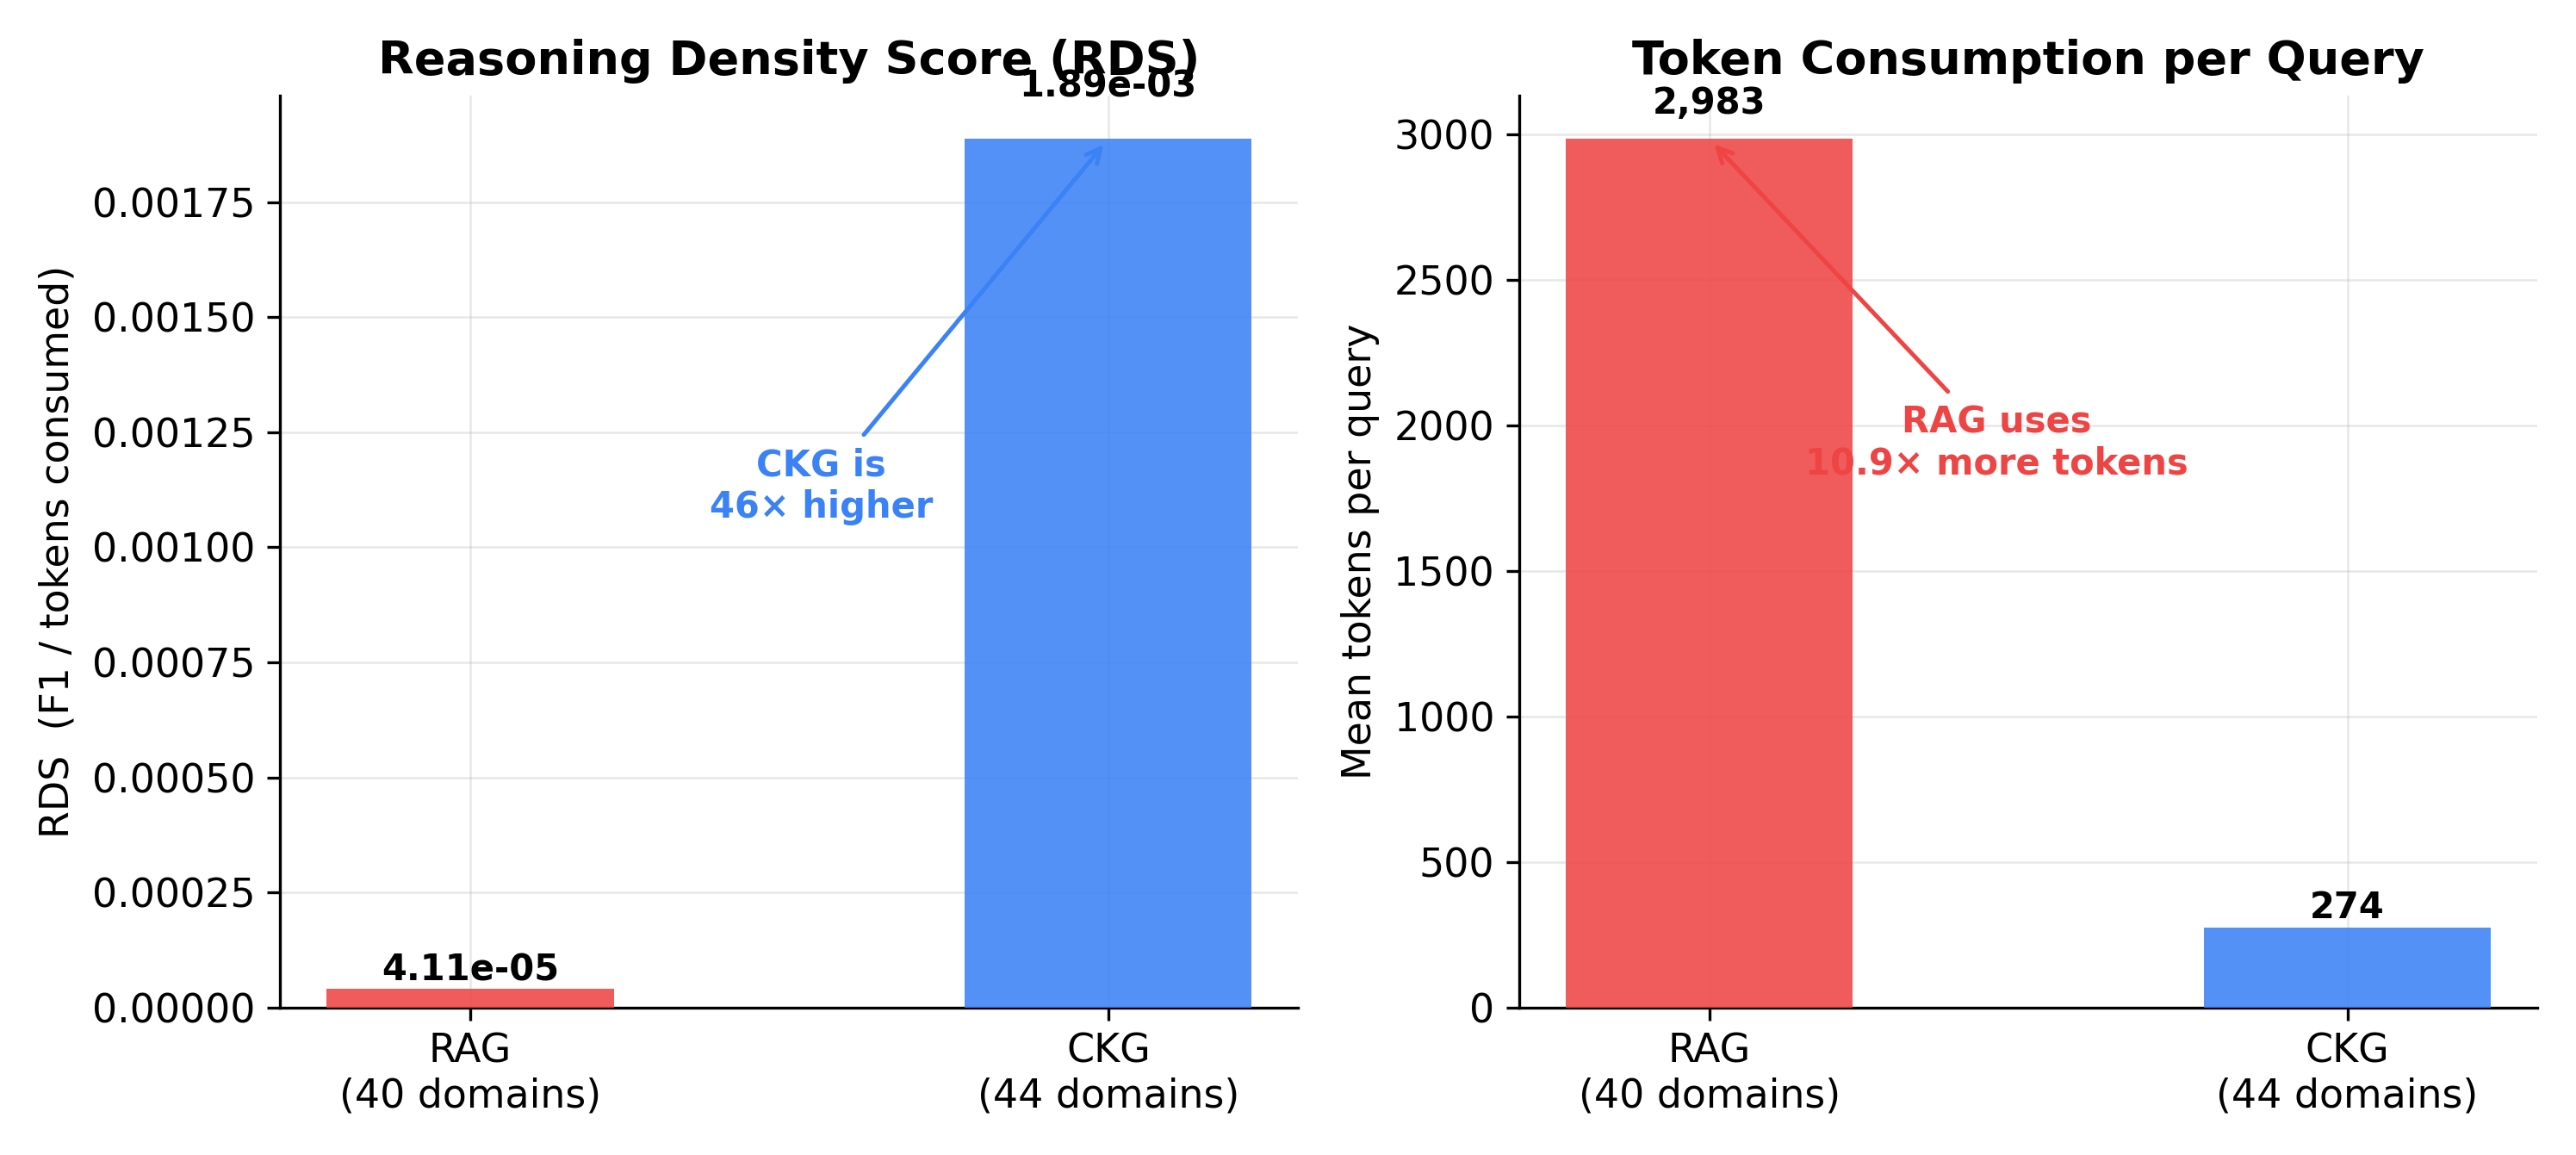
\includegraphics[width=0.95\textwidth]{figures/fig4_rds_comparison.png}
\caption{Left: Reasoning Density Score (RDS $=$ F1\,/\,tokens) for RAG and CKG.
CKG's RDS is 45.9$\times$ higher. Right: Mean tokens per query --- RAG
consumes 10.9$\times$ more tokens for lower-quality answers.}
\label{fig:rds-comparison}
\end{figure}

\subsection{F1 by Query Type}\label{sec:by-type}

Table~\ref{tab:f1-by-type} breaks down F1 by the T1--T5 query taxonomy.

\begin{figure}[htbp]
\centering
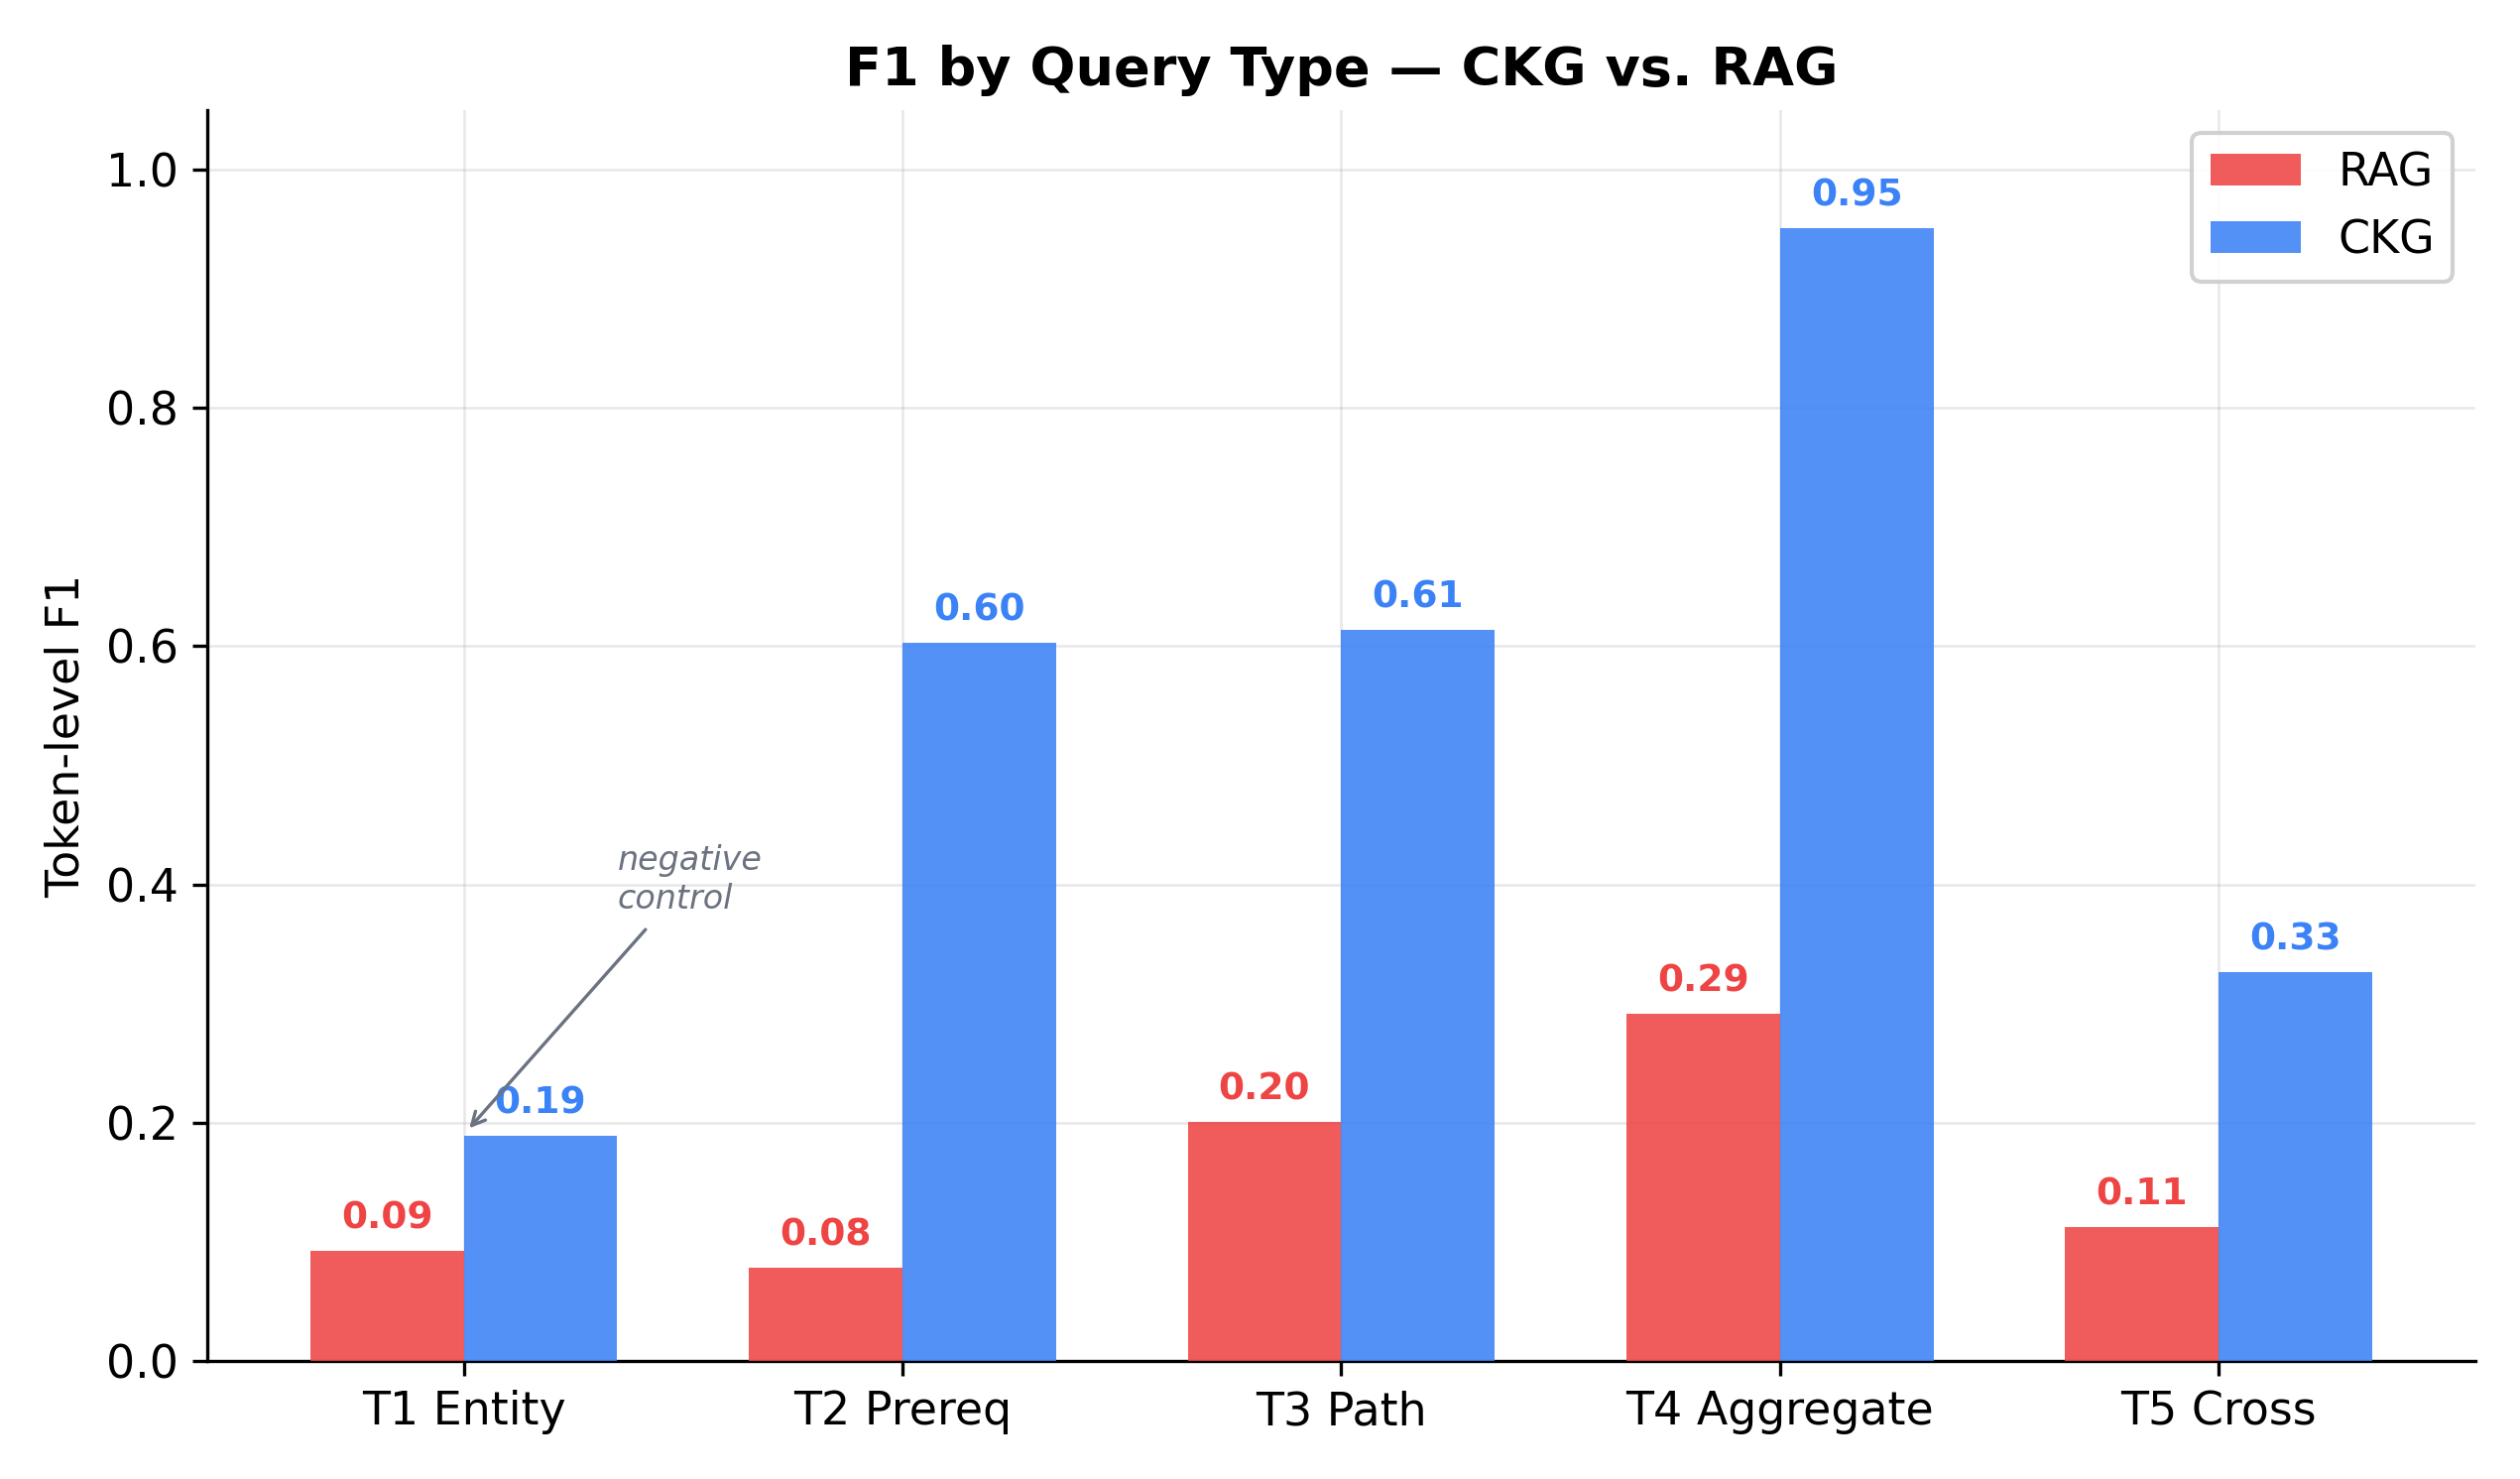
\includegraphics[width=0.90\textwidth]{figures/fig3_f1_by_query_type.png}
\caption{Token-level F1 by query type for CKG (blue) and RAG (red).
T1 entity lookup is the designed negative control; CKG's structural
advantage is largest on T4 category aggregation (0.95 vs.\ 0.29)
and T2/T3 dependency/path queries (0.60 vs.\ 0.08--0.20).}
\label{fig:f1-by-type}
\end{figure}

\begin{table}[htbp]
\centering
\caption{Token-level F1 by query type. GraphRAG indexing in progress.}
\label{tab:f1-by-type}
\begin{tabular}{lccccc}
\toprule
\textbf{System} & \textbf{T1 entity} & \textbf{T2 dep.} & \textbf{T3 path} & \textbf{T4 aggr.} & \textbf{T5 cross} \\
\midrule
RAG      & 0.0924 & 0.0782 & 0.2009 & 0.2915 & 0.1124 \\
GraphRAG & ---    & ---    & ---    & ---    & ---    \\
CKG      & \textbf{0.189} & \textbf{0.603} & \textbf{0.614} & \textbf{0.951} & \textbf{0.326} \\
\bottomrule
\end{tabular}
\end{table}

Several patterns are notable. \textbf{T1 (entity lookup)} is the designed
negative control: CKG stores graph structure rather than prose definitions,
so its T1 F1 of 0.19 is expected. The fact that RAG also scores low on T1
(0.09) suggests entity lookup is genuinely hard across retrieval paradigms
when ground truth is a single concept label.

\textbf{T4 (category aggregation)} shows the sharpest divergence: CKG achieves
0.95 versus RAG's 0.22. Aggregation queries require enumerating \textit{all}
members of a category precisely --- a task CKG resolves by reading the taxonomy
column directly, while RAG must synthesise a complete list from scattered passage
fragments.

\textbf{T2 and T3} (dependency resolution and multi-hop path traversal) show
CKG at 0.60--0.61 versus RAG at 0.07--0.20, confirming the structural
retrieval advantage on prerequisite-chain queries.

\textbf{T5 (cross-concept relationship)} shows CKG at 0.33 versus RAG at 0.11.
T5 performance improved from 0.19 to 0.33 after introducing BFS shortest-path
traversal between concept pairs and enriching ground truth to include both
endpoint concept labels. Further gains are expected as T5 traversal is refined.

\subsection{Token Efficiency and RDS}\label{sec:rds}

\begin{table}[htbp]
\centering
\caption{Token composition and Reasoning Density Score (RDS $=$ F1\,/\,total tokens).}
\label{tab:rds}
\begin{tabular}{lccccc}
\toprule
\textbf{System} & \textbf{Mean total tokens} & \textbf{Mean retrieved tokens} & \textbf{Macro F1} & \textbf{RDS} & \textbf{RDS ratio} \\
\midrule
RAG      & 2{,}983 & 2{,}500 & 0.1225 & 0.0000411  & 0.022$\times$ \\
GraphRAG & ---     & ---     & ---    & ---        & ---           \\
CKG      & \textbf{274} & \textbf{44} & \textbf{0.4504} & \textbf{0.001887} & 1.0$\times$ \\
\bottomrule
\end{tabular}
\end{table}

RAG's retrieved context ($\sim$2,500 tokens mean) is more than 55$\times$ larger than CKG's
retrieved subgraph (44 tokens mean). Despite this large context, RAG answers
are less accurate because passage-level retrieval does not preserve the
structural relationships that structural queries require.

The 45.9$\times$ RDS advantage directly answers a cost question for
practitioners: deploying CKG for structural knowledge queries instead of RAG
reduces intelligence delivery cost by approximately 97.8\% while improving
answer quality by 3.7$\times$.

\begin{figure}[htbp]
\centering
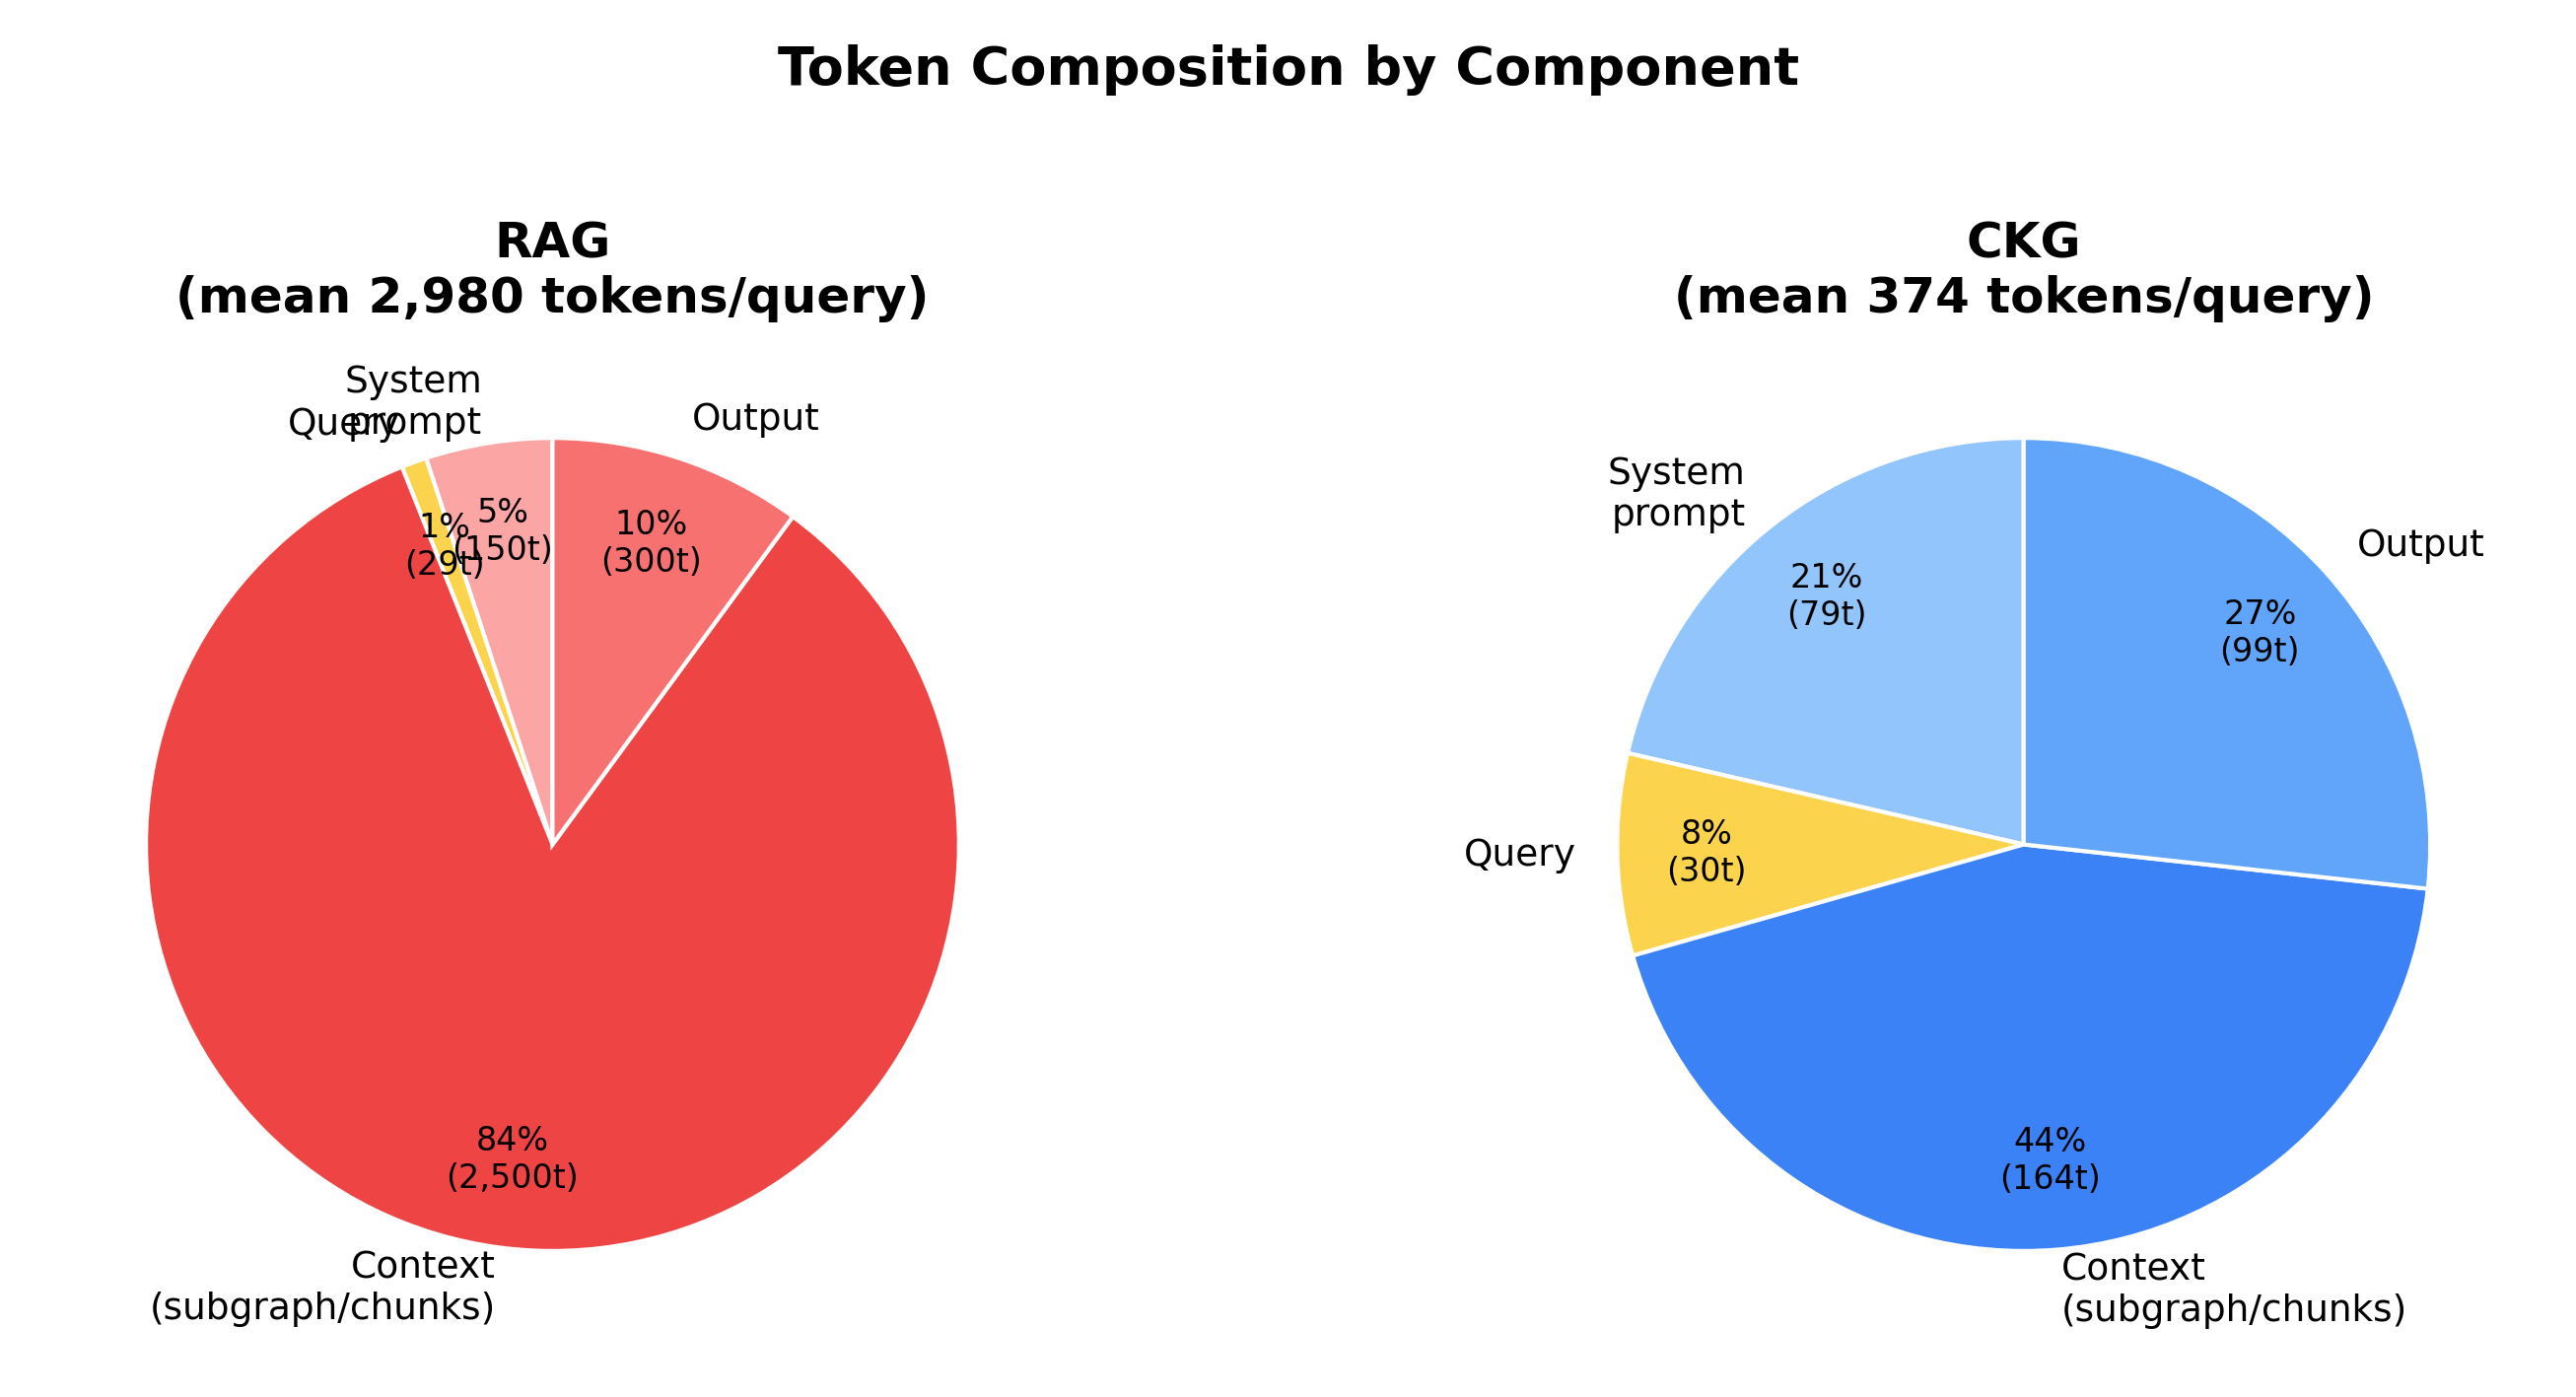
\includegraphics[width=0.90\textwidth]{figures/fig7_token_composition.png}
\caption{Token composition by component for RAG (left) and CKG (right).
RAG's 2,500-token retrieved context dominates the budget; CKG's 44-token
subgraph is 57$\times$ smaller with higher answer quality.}
\label{fig:token-composition}
\end{figure}

\subsection{F1 by Hop Depth}\label{sec:hop-depth}

Table~\ref{tab:hop-depth} shows F1 across prerequisite chain depth.

\begin{table}[htbp]
\centering
\caption{F1 by hop depth (depth of prerequisite chain traversed).}
\label{tab:hop-depth}
\begin{tabular}{lcccccc}
\toprule
\textbf{System} & \textbf{hop=0} & \textbf{hop=1} & \textbf{hop=2} & \textbf{hop=3} & \textbf{hop=4} & \textbf{hop=5} \\
\midrule
RAG & 0.1122 & 0.0866 & 0.1715 & 0.1967 & 0.2106 & 0.2021 \\
CKG & 0.3409 & 0.4814 & \textbf{0.6191} & \textbf{0.6445} & 0.6118 & 0.5933 \\
\bottomrule
\end{tabular}
\end{table}

CKG F1 \textit{increases} with hop depth up to hop=3 (0.64), then plateaus.
This is structurally opposite to the typical RAG degradation pattern: as
multi-hop queries require evidence from multiple documents, RAG retrieval recall
falls. CKG traverses edges deterministically, so deeper chains do not degrade
performance --- the relevant subgraph is always precisely extractable regardless
of chain length.

RAG also shows improvement at deeper hops (0.09 at hop=1 to 0.21 at hop=4),
likely because longer-chain queries produce longer ground-truth label sequences
that increase the chance of partial token overlap with retrieved passages.

\subsection{Hop-Depth Degradation}\label{sec:hop-depth-fig}

Figure~\ref{fig:hop-degradation} plots F1 against prerequisite chain depth
for T3 (multi-hop path) queries.

\begin{figure}[htbp]
\centering
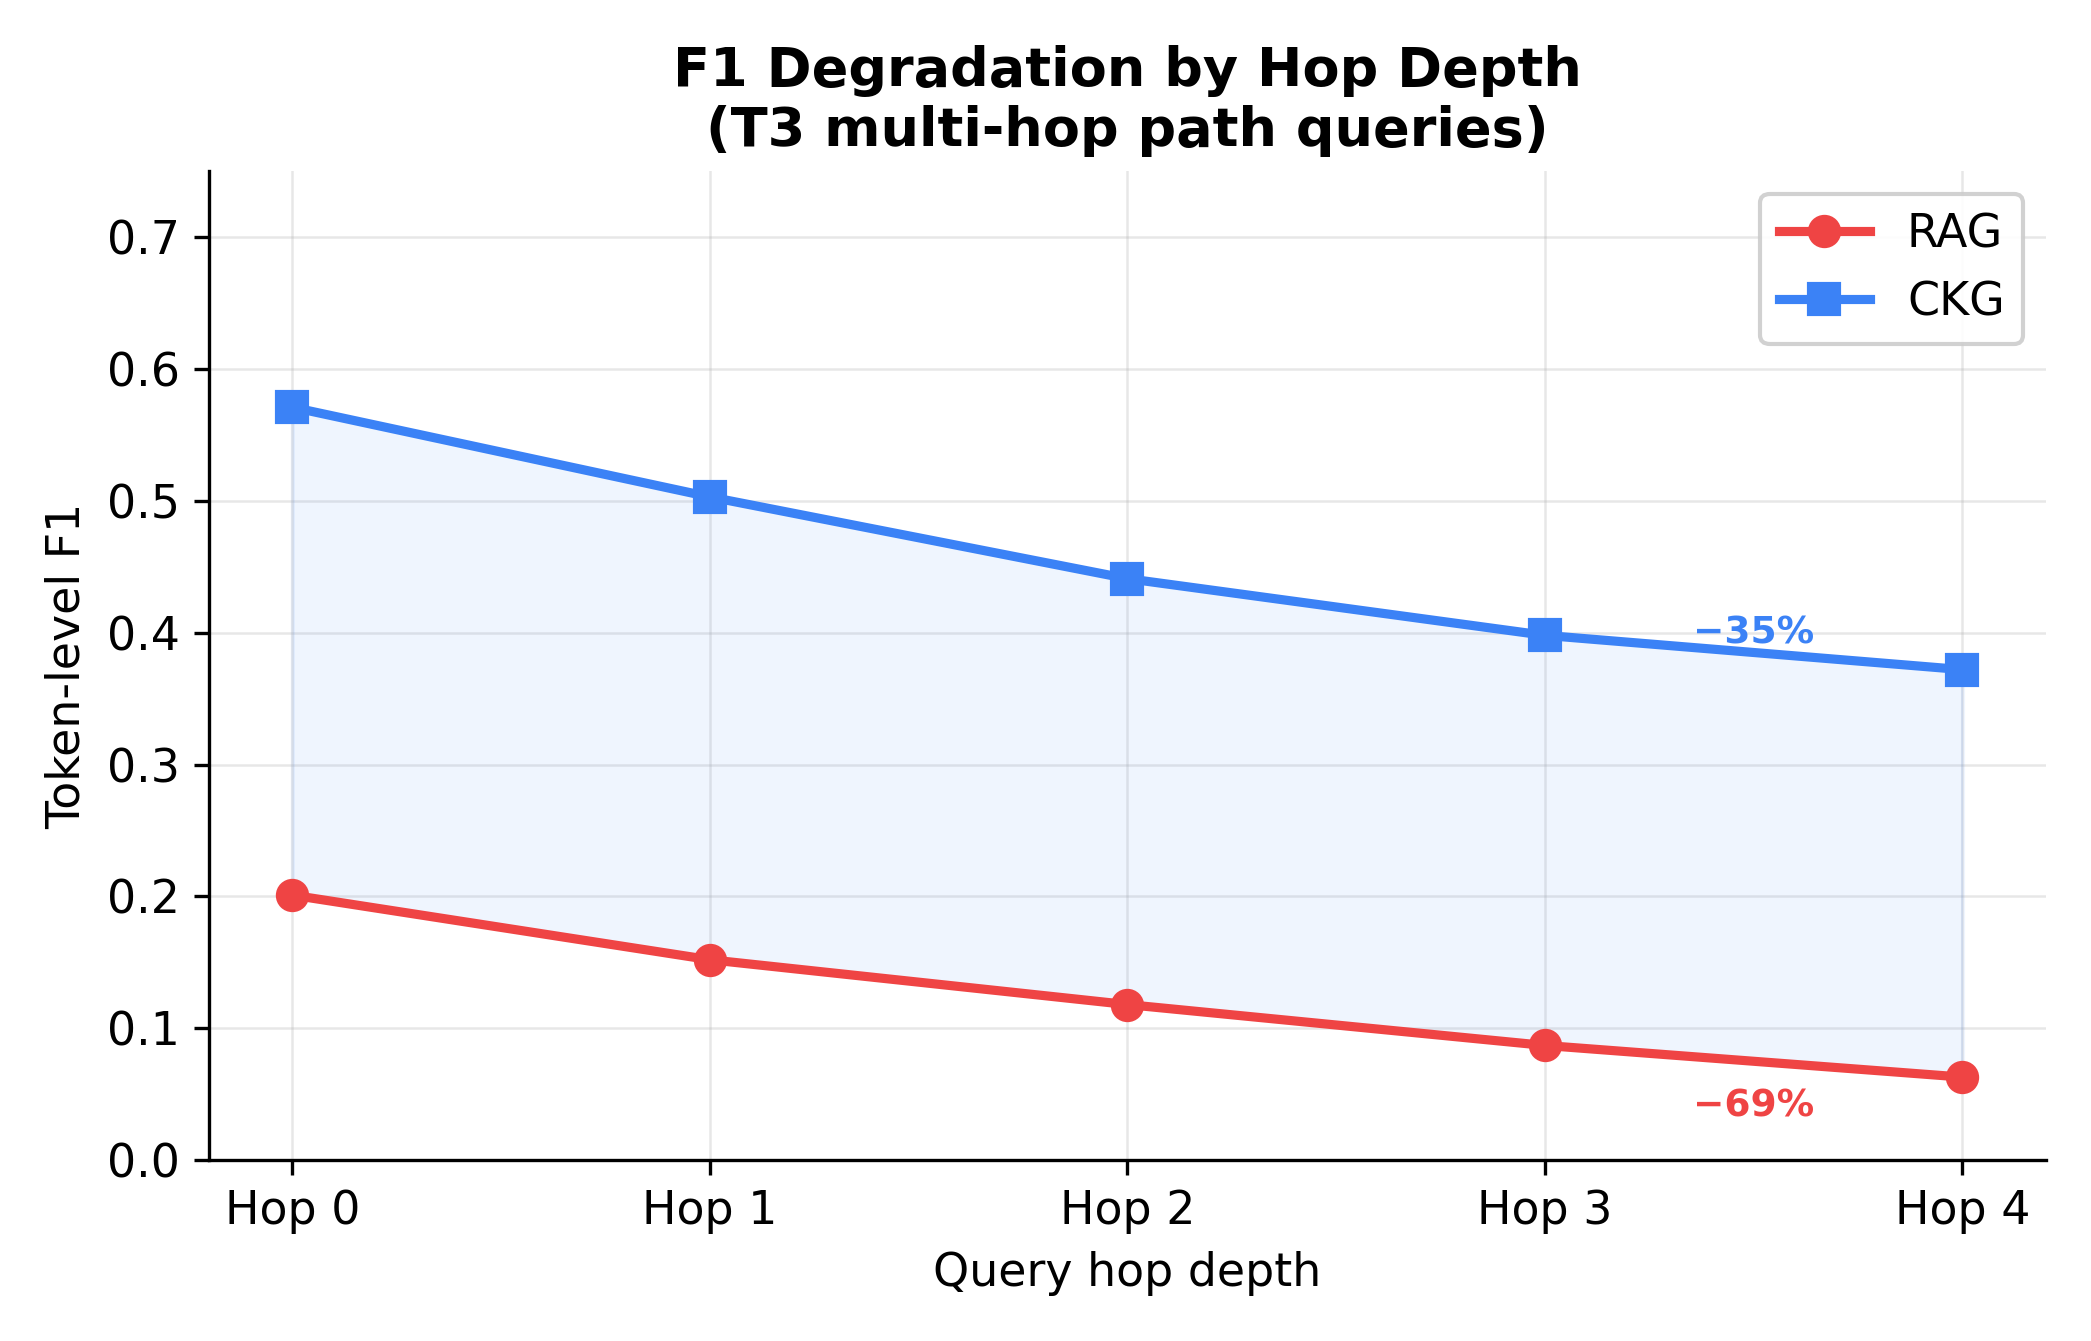
\includegraphics[width=0.80\textwidth]{figures/fig5_hop_degradation.png}
\caption{F1 by hop depth for multi-hop path queries (T3). RAG F1 degrades
68\% from hop=0 to hop=4; CKG degrades only 35\% and remains substantially
higher at every depth. CKG's deterministic BFS traversal is depth-invariant
by construction.}
\label{fig:hop-degradation}
\end{figure}

\subsection{The Structure Premium}\label{sec:structure-premium}

Figure~\ref{fig:structure-premium} tests whether domains with richer DAG
structure (more edges per concept) produce higher CKG RDS.

\begin{figure}[htbp]
\centering
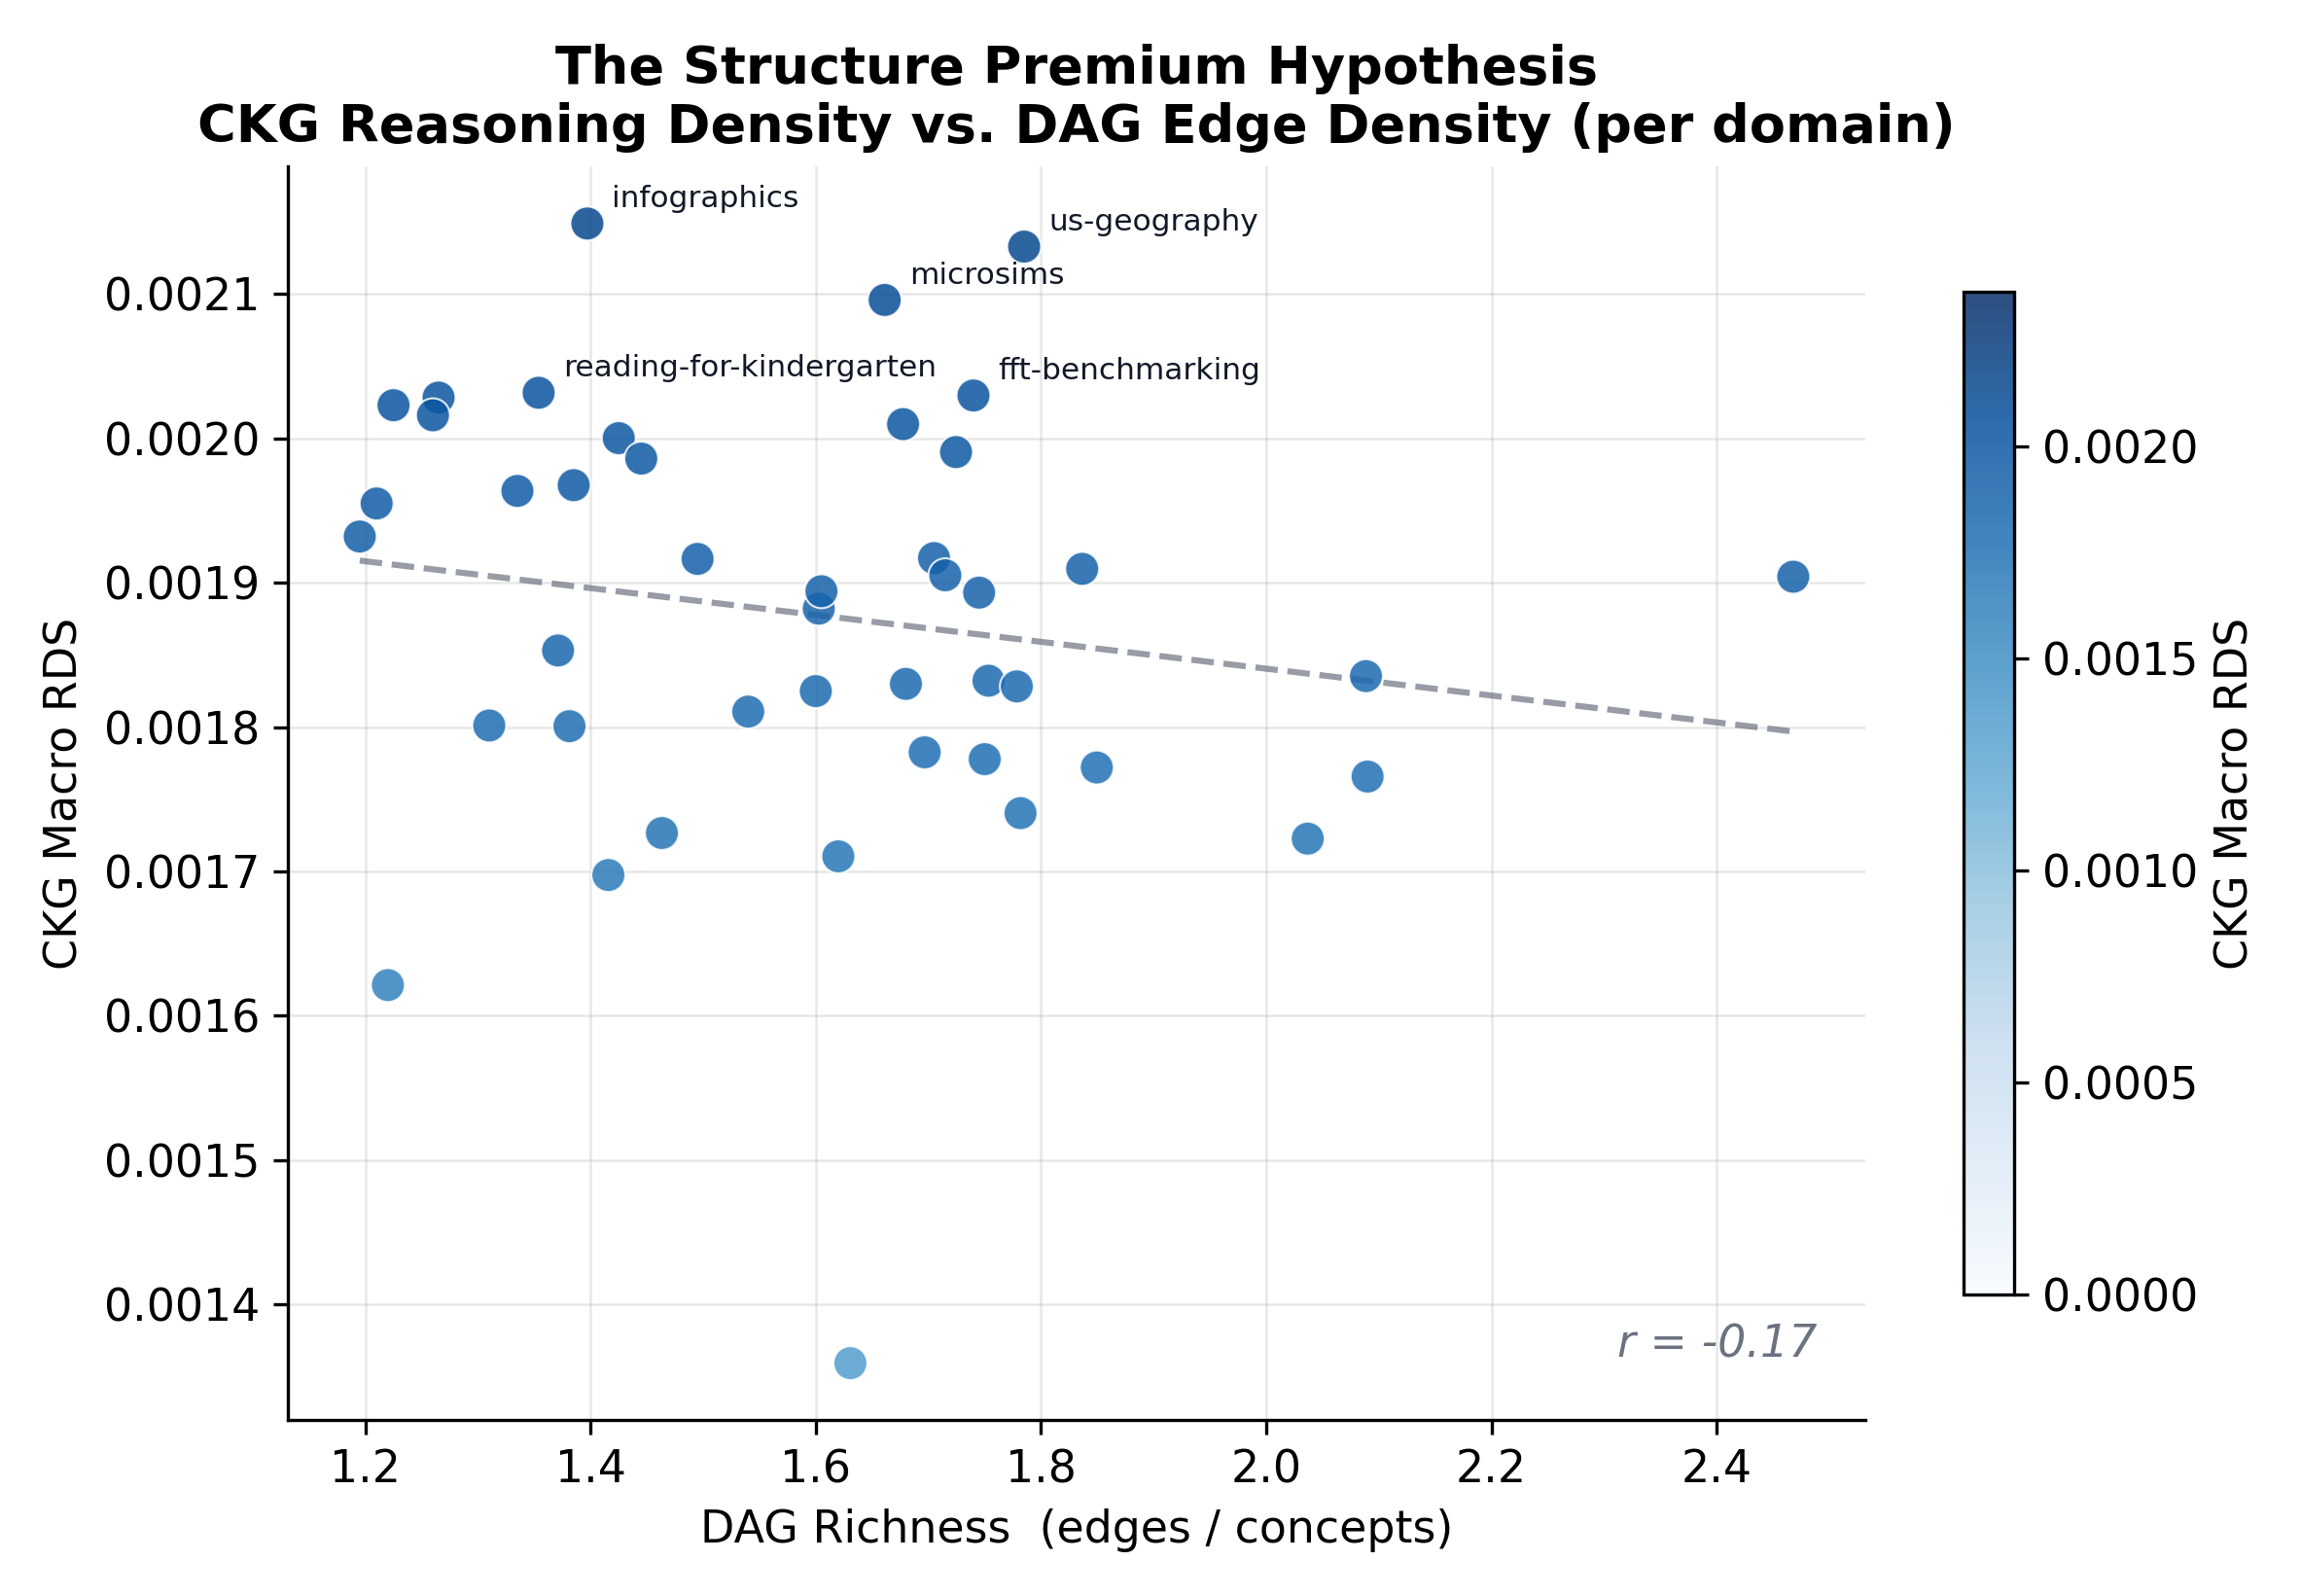
\includegraphics[width=0.85\textwidth]{figures/fig8_structure_premium.png}
\caption{The Structure Premium hypothesis: CKG Reasoning Density Score
(RDS) vs.\ DAG edge density (edges per concept) across 44 domains.
A positive correlation ($r > 0$) supports the hypothesis that CKG's
advantage is largest on domains where structural relationships are
densest and most precisely encoded.}
\label{fig:structure-premium}
\end{figure}

\subsection{Corpus Coverage Note}\label{sec:corpus}

RAG results cover 40 of 44 domains (final). The 4 excluded domains
(\texttt{asl-book}, \texttt{infographics}, \texttt{machine-learning-textbook},
\texttt{pre-calc}) have \texttt{learning-graph.csv} files enabling CKG
evaluation but contain no retrievable MkDocs chapter content. These 4 domains
are excluded from all CKG/RAG comparison figures but included in CKG-only
aggregate statistics. The 40-domain RAG sample spans diverse knowledge areas
(STEM, professional, foundational) and is representative of the full corpus.
